Qui di seguito è riportato uno schema logico del database mediante modello Relazionale.
\begin{figure}[htp]
\centering
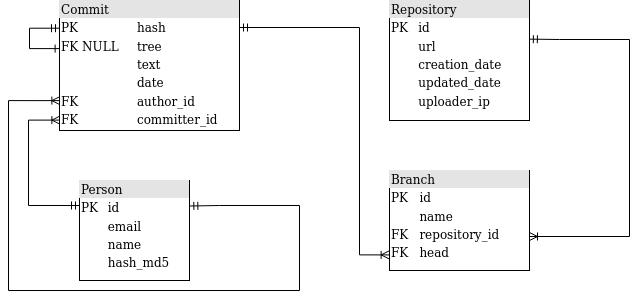
\includegraphics[scale=0.70]{data/relation.png}
\caption{Modello relazionale}
\label{}
\end{figure}

Come si può ben vedere sono state fatte delle modifiche:
\begin{itemize}
\item Repository: aggiunte le date di creazione e modifica;
\item Branch: ha un suo id come PK, in modo da accedervi più facilmente tramite backend. Questo perché i branch permettono anche lo slash nel nome, cosa che andrebbe a creare errore se passato nell'endpoint;
\item Commit: ha un campo \verb|tree| che si riferisce al parent: può ovviamente essere null. Dato che il commit può essere scritto da massimo 2 persone, ho preferito aggiungere i campi \verb|author_id| e \verb|committer_id|;
\item Person: ha un campo \verb|hash_md5| che calcola l'MD5\footnote{https://en.wikipedia.org/wiki/MD5} dell'email una volta sola: usato per il Gravatar\footnote{https://en.gravatar.com/};
\end{itemize}

\section{Considerazioni}
Il numero di elementi presenti nella tabella \verb|Commit| saranno molti: molti di più rispetto a quelli presenti in \verb|Person|. Questo perché si presuppone che aggiunta una \verb|Repository| verranno aggiunti i commit di un determinato \verb|Branch| che, a meno di repositories particolari, non avranno un numero di contributors molto maggiore rispetto a quello dei commits.
\paragraph{Esempio} Il progetto Rust\footnote{https://github.com/rust-lang/rust} ha | mentre scrivo questo documento | \textbf{139,832} commits e \textbf{3,203} contributors.\\\\
\noindent
Se seguiamo il progetto citato sopra e lanciamo una query d'esempio:
\paragraph{Query 1} Selezionare hash, testo, data, nome ed email di autore e committente.\\\\\noindent
Per eseguire la \textit{Query 1} dovremmo realizzare 2 join a \verb|Person| per ogni record. Se togliessimo le due foreign key avremmo un risparmio considerevole: non faccio il calcolo perché è facile da vedere.
\paragraph{Insert 1} Inserire un nuovo commit.\\\\\noindent
Per eseguire l'operazione \textit{Insert 1} bisognerebbe cercare su \verb|Person| se esiste già un elemento associato a quell'email e quel nome: se esiste lo legge, altrimenti lo crea. Cercare su \verb|Person| se esiste già un elemento associato a quell'email e quel nome: se esiste lo legge, altrimenti lo crea. Infine scrivere all'interno di \verb|Commit|. La foreign key \verb|tree| è irrilevante perché fa riferimento ad un hash di un commit già esistente, quindi non c'è bisogno di controllo.

Se volessimo sapere a quale repository si riferisce un commit bisognerebbe cercare il \verb|Branch| che ha un \verb|head| che è uguale all'\verb|hash| e in caso negativo procedere ricorsivamente per \verb|tree|. Se siamo fortunati becchiamo il \verb|Commit| che è \verb|head| del \verb|Branch| e ce ne usciamo con 1 giunzione, altrimenti il costo in SQL sarebbe quello di una chiamata ricorsiva tale che, partendo da un commit \verb|c1| vada a cercare il commit appartenente al \verb|tree| e così via. Ora, eseguire una query del genere 1 volta per apertura della pagina del commit\footnote{Ad esempio con endpoint \textit{/api/commit/2cde51fbd0f310c8a2c5f977e665c0ac3945b46d/}} non è un problema; il problema è quando vogliamo vedere la repository associata ad \underline{ognuno} dei commit. Certo, si potrebbe risolvere lato codice, ma questo è un progetto per il corso di Basi di Dati, quindi dobbiamo risolverlo tramite chiamata SQL.

\section{Schema logico finale}
In Figura 4.2 vi è una versione revisionata del modello Relazionale.

Possiamo notare svariate modifiche apportate:
\begin{itemize}
\item I \verb|Commit| non puntano direttamente a 2 record di \verb|Person|: le foreign key fanno riferimento solo alle emails. Questo perché Git considera diverse due persone con stessa email ma nome diverso. A noi interessa sapere l'hash MD5 per avere il Gravatar associato all'email. Se poi cambia nome, l'immagine dovrà essere comunque sempre la stessa. Quando non ci interessa avere l'avatar, inoltre, non dobbiamo fare giunzioni alla nuova tabella \verb|Email|.

Se ci serve avere l'hash potremmo prima fare una \verb|SELECT| delle email associate all'hash e utilizzare un hash per associare, lato client, l'hash alla singola email. Quindi non fare giunzioni. Ma questo lato client, quindi la tabella resta per il funzionamento tramite SQL.

\item Al \verb|Commit| è associata la url della \verb|Repository|. Dato che la PK della \verb|Repository| è l'\verb|id|, il campo \verb|url| è diventanto \verb|UNIQUE|. Cosa che a noi sta più che bene, dato che non vogliamo \verb|Repository| duplicate.

\item Anche il campo \verb|hash_md5| è \verb|UNIQUE|. In realtà è una cosa extra, dato che, se dovessimo riscontrare un'errore del genere le alternative sono due: o in realtà l'email esiste già nel database oppure abbiamo trovato un'altra parola che ha come risultato dell'hash MD5, una già esistente.
\end{itemize}

\begin{figure}[htp]
\centering
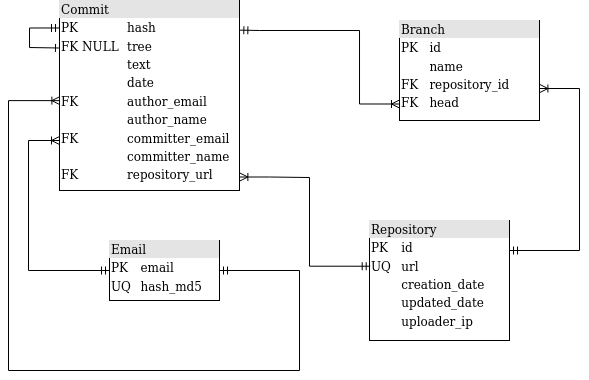
\includegraphics[scale=0.7]{data/relation_final.png}
\caption{Modello relazionale finale}
\label{}
\end{figure}